\documentclass[UTF-8]{ctexart} 
\usepackage[a4paper,left=2cm,right=2cm,top=2.5cm,bottom=2.5cm]{geometry}
\usepackage{amsmath,bm,amssymb}
\usepackage{siunitx}
\usepackage{physics}
\usepackage{lmodern}
\usepackage{tikz}
\usepackage{cutwin}
\usepackage{fancyhdr}
\usepackage{caption}
\usepackage{enumitem}
\usepackage{upgreek}
\usepackage{circuitikz}
\usepackage{mathrsfs}
\usetikzlibrary{snakes,fadings}
\usetikzlibrary{decorations.pathmorphing}
\usetikzlibrary{shapes}

\tikzfading[name=fade left, left color=transparent!30, right color=transparent!70]

\captionsetup{labelformat=empty}
%\renewcommand\thefigure{\theenumi}
\makeatletter
\renewcommand*\maketitle{
    \begin{center}
        \bfseries
        {\Large \@title \par}
        \vskip 1em
        {\global\let\author\@empty}
        {\global\let\date\@empty}
    \end{center}
  \setcounter{footnote}{0}
}
\newcommand{\mlabel}[2]{#2\def\@currentlabel{#2}\label{#1}}
\newcommand{\cube}[5]{
    \pgfmathsetmacro{\cubex}{#2}
    \pgfmathsetmacro{\cubey}{#3}
    \pgfmathsetmacro{\cubez}{#4}
    \filldraw[#5!50,join=round] #1 -- ++(-\cubex,0,0) -- ++(0,-\cubey,0) -- ++(\cubex,0,0) -- cycle;
    \filldraw[#5,join=round] #1 -- ++(0,0,-\cubez) -- ++(0,-\cubey,0) -- ++(0,0,\cubez) -- cycle;
    \filldraw[#5!80,join=round] #1 -- ++(-\cubex,0,0) -- ++(0,0,-\cubez) -- ++(\cubex,0,0) -- cycle;
}
\renewcommand\theenumi{S-\arabic{enumi}}
\renewcommand\labelenumi{\theenumi}
\sisetup{inter-unit-product = \ensuremath { { } \cdot { } } }
\newcommand{\csi}[2]{ \SI{#1}{#2}}
\makeatother

\pagestyle{fancy}
\fancyhf{}
\cfoot{\thepage}
\renewcommand\headrulewidth{0pt}
\title{第7章\ 恒定磁场}
\author{叶旺全\\大学物理教研室}

\begin{document} 
\maketitle
\begin{enumerate}
    % \item[\mlabel{itm:a}{5-6}] 自定义label引用参考
    \item[7-8] 两个同轴圆柱面导体的长度均为\csi{20}{\meter},内圆柱面的半径为\csi{3.0}{\mm},外圆柱面的半径为\csi{9.0}{\mm}。
         若两圆柱面之间有\csi{10}{\uA}的电流沿径向流过,求通过半径为\csi{6.0}{\mm}的圆柱面的电流密度。
    
    \item[\mlabel{itm:10}{7-10}] 如图所示,两根导线沿半径方向接到铁环的\(a\)、\(b\)两点,并与很远处的电源相连接。
        求环心点\(O\)的磁感强度。
        \begin{figure}[htbp]
            \centering
            \begin{minipage}[b]{0.4\textwidth}
                \centering
                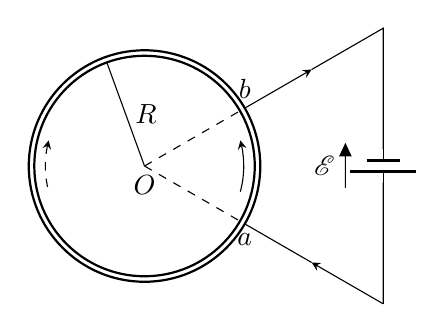
\begin{tikzpicture}[scale=0.7]
                    \draw[thick] (0,0) circle (2);
                    \draw[thick] (0,0) circle (2.1);
                    \draw (0,0) node[below]{\(O\)} -- node[right]{\(R\)} (110:2);
                    \draw[dashed,stealth-] (165:1.8) arc (165:195:1.8);
                    \draw[-stealth] (-15:1.8) arc (-15:15:1.8);
                    \draw[dashed] (0,0) -- (30:2.1);
                    \draw[-stealth] (30:2.1) node[above]{\(b\)} -- (30:3.5);
                    \draw[dashed] (0,0) -- (-30:2.1);
                    \draw (-30:2.1) node[below]{\(a\)} -- (-30:3.5);
                    \draw[stealth-] (-30:3.5) -- (-30:5);
                    \draw (-30:5) to[battery1=\(\mathscr{E}\)] (30:5) -- (30:3.5);
                \end{tikzpicture}
                \caption{\ref{itm:10} 题图}
            \end{minipage}
        \end{figure}

    \item[\mlabel{itm:12}{7-12}] 载流导线形状如图所示(图中直线部分导线延伸到无限远),求点\(O\)的磁感强度\(\bm{B}\)。
        \begin{figure}[htbp]
            \centering
            \begin{minipage}[b]{0.3\textwidth}
                \centering
                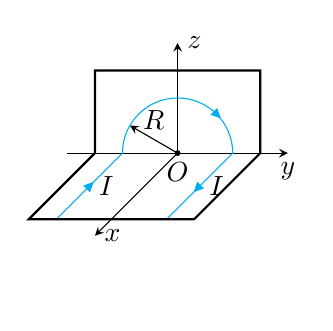
\begin{tikzpicture}[scale=0.7]
                    \draw[transparent] (0,0) -- (0,-2.7);
                    \draw[-stealth] (-2,0) -- (2,0) node[below]{\(y\)};
                    \draw[-stealth] (0,0) -- (0,2) node[right]{\(z\)};
                    \draw[-stealth] (0,0) -- (-1.5,-1.5) node[right]{\(x\)};
                    \fill (0,0) node[below]{\(O\)} circle (1.5pt);
                    \draw[-stealth] (0,0) -- node[above]{\(R\)} (150:1);
                    \draw[cyan] (-2.2,-1.2)-- node[currarrow,scale=0.7,rotate=45,color=cyan]{} 
                        (180:1) arc (180:0:1) node[near end,currarrow,scale=0.7,rotate=-45,color=cyan]{} 
                        -- node[currarrow,scale=0.7,rotate=-135,right,color=cyan]{} (-0.2,-1.2) ;
                    \node[right] at (0.4,-0.6) {\(I\)};
                    \node[right] at (-1.6,-0.6) {\(I\)};
                    \draw[thick] (-1.5,0) -- (-1.5,1.5) -- (1.5,1.5) -- (1.5,0) 
                        -- (0.3,-1.2) -- (-2.7,-1.2) -- cycle;
                \end{tikzpicture}
                \caption{(a)}
            \end{minipage}
            \begin{minipage}[b]{0.3\textwidth}
                \centering
                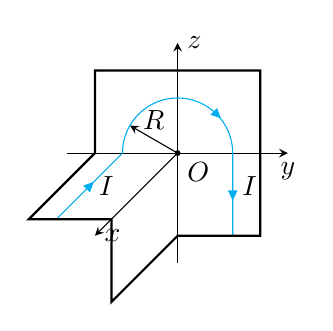
\begin{tikzpicture}[scale=0.7]
                    \draw[-stealth] (-2,0) -- (2,0) node[below]{\(y\)};
                    \draw[-stealth] (0,-2) -- (0,2) node[right]{\(z\)};
                    \draw[-stealth] (0,0) -- (-1.5,-1.5) node[right]{\(x\)};
                    \fill (0,0) node[below right]{\(O\)} circle (1.5pt);
                    \draw[-stealth] (0,0) -- node[above]{\(R\)} (150:1);
                    \draw[cyan]  (-2.2,-1.2) -- node[currarrow,scale=0.7,rotate=45,color=cyan]{} (180:1) 
                        arc (180:0:1) node[near end,currarrow,scale=0.7,rotate=-45,color=cyan]{} 
                        -- node[currarrow,scale=0.7,rotate=-90,color=cyan]{} (1,-1.5);
                    \node[right] at (1,-0.6) {\(I\)};
                    \node[right] at (-1.6,-0.6) {\(I\)};
                    \draw[thick] (-1.5,0) -- (-1.5,1.5) -- (1.5,1.5) -- (1.5,-1.5) 
                        -- (0,-1.5) -- (-1.2,-2.7) -- (-1.2,-1.2) -- (-2.7,-1.2) -- cycle;
                \end{tikzpicture}
                \caption{(b)}
            \end{minipage}
            \begin{minipage}[b]{0.3\textwidth}
                \centering
                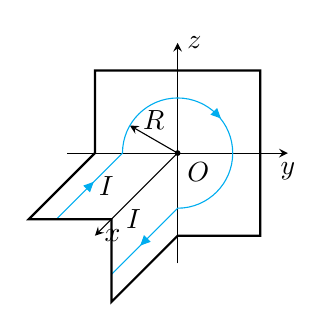
\begin{tikzpicture}[scale=0.7]
                    \draw[-stealth] (-2,0) -- (2,0) node[below]{\(y\)};
                    \draw[-stealth] (0,-2) -- (0,2) node[right]{\(z\)};
                    \draw[-stealth] (0,0) -- (-1.5,-1.5) node[right]{\(x\)};
                    \fill (0,0) node[below right]{\(O\)} circle (1.5pt);
                    \draw[-stealth] (0,0) -- node[above]{\(R\)} (150:1);
                    \draw[cyan]  (-2.2,-1.2) -- node[currarrow,scale=0.7,rotate=45,color=cyan]{} (180:1) 
                        arc (180:0:1) node[near end,currarrow,scale=0.7,rotate=-45,color=cyan]{} 
                        arc (0:-90:1) -- node[currarrow,scale=0.7,rotate=-135,color=cyan]{} (-1.2,-2.2);
                    \node at (-0.8,-1.2) {\(I\)};
                    \node[right] at (-1.6,-0.6) {\(I\)};
                    \draw[thick] (-1.5,0) -- (-1.5,1.5) -- (1.5,1.5) -- (1.5,-1.5) 
                        -- (0,-1.5) -- (-1.2,-2.7) -- (-1.2,-1.2) -- (-2.7,-1.2) -- cycle;
                \end{tikzpicture}
                \caption{(c)}
            \end{minipage}
            \caption{\ref{itm:12} 题图}
        \end{figure}

    \item[\mlabel{itm:13}{7-13}] 如图所示,一个半径为\(R\)的无限长半圆柱面导体,沿长度方向的电流\(I\)在柱面上均匀分布,求半圆柱面轴线
        \(OO^\prime\)上的磁感强度。
        \begin{figure}[htbp]
            \centering
            \begin{minipage}[b]{0.4\textwidth}
                \centering
                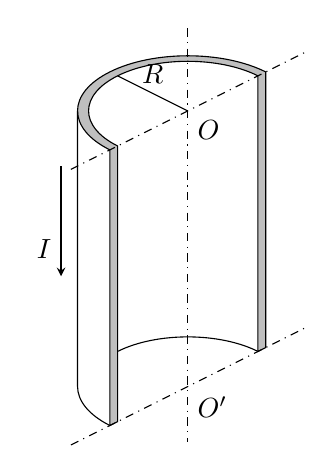
\begin{tikzpicture}[scale=0.7]
                    [dashdotted/.style={dash pattern={on 10pt off 2pt on 2pt off 2pt}}]
                    \draw (45:1.8 and 0.9)++(0,-5) arc (45:135:1.8 and 0.9);
                    \draw[fill = lightgray] (225:2 and 1) arc (225:45:2 and 1) -- ++(0,-5) -- ++(225:0.2 and 0.1)
                        -- ++(0,5) arc (45:225:1.8 and 0.9) -- ++(0,-5) -- ++(225:0.2 and 0.1)
                        -- cycle;
                    \draw (180:2 and 1) -- ++(0,-5) arc (180:225:2 and 1);
                    \draw[dashdotted] (0,1.5) -- (0,-6);
                    \draw[dashdotted] (225:3 and 1.5) -- (45:3 and 1.5);
                    \draw[dashdotted] (225:3 and 1.5)++(0,-5) -- +(45:6 and 3);
                    \draw (0,0) node[below right]{\(O\)} -- node[above]{\(R\)} (135:1.8 and 0.9);
                    \draw[-stealth] (180:2.3 and 1.15)++(0,-1) -- ++(0,-2) node[near end,left]{\(I\)};
                    \node[below right] at (0,-5) {\(O^\prime\)};
                \end{tikzpicture}
                \caption{\ref{itm:13} 题图}
            \end{minipage}
        \end{figure}
    
    \item[\mlabel{itm:17}{7-17}] 有一同轴电缆,其尺寸如图所示。两导体中电流均为\(I\),但电流的流向相反,导体的磁性可不考虑。
        试计算以下各处的磁感强度:(1)\(r<R_1\);(2)\(R_1<r<R_2\);(3)\(R_2<r<R_3\);(4)\(r>R_3\)。画出\(B-r\)图线。
    
    \item[\mlabel{itm:20}{7-20}] 电流\(I\)均匀地流过半径为\(R\)的圆形长直导线,试计算单位长度导线中通过图中所示剖面的磁通量。
    \begin{figure}[htb]
        \centering
        \begin{minipage}[b]{0.4\textwidth}
            \centering
            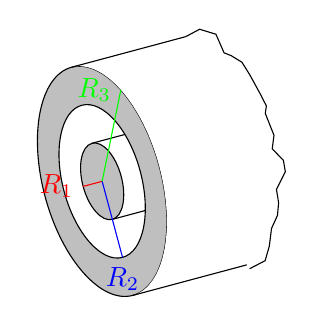
\begin{tikzpicture}[decoration={random steps,segment length=5pt,amplitude=2pt},rotate=15]
                \draw (90:0.25 and 0.5) -- ++(0.6,0) arc (90:-90:0.25 and 0.5) -- ++(-0.6,0);
                \draw[fill=lightgray,even odd rule] (0,0) ellipse (0.25 and 0.5) (0,0) ellipse (0.5 and 1)
                    (0,0) ellipse (0.75 and 1.5);
                \fill[fill=white] (90:0.75 and 1.5) -- ++(1.5,0) arc (90:-90:0.75 and 1.5) -- ++(-1.5,0) arc (-90:90:0.75 and 1.5);
                \draw (0,1.5) -- ++(1.5,0);
                \draw (0,-1.5) -- ++(1.5,0);
                \draw[decorate] (1.5,1.5) arc (90:-90:0.75 and 1.5);
                \draw[red] (0,0) -- (180:0.25 and 0.5) node[left]{\(R_1\)};
                \draw[blue] (0,0) -- (270:0.5 and 1) node[below]{\(R_2\)};
                \draw[green] (0,0) -- (45:0.75 and 1.5) node[left]{\(R_3\)};
            \end{tikzpicture}
            \caption{\ref{itm:17} 题图}
        \end{minipage}
        \begin{minipage}[b]{0.4\textwidth}
            \centering
            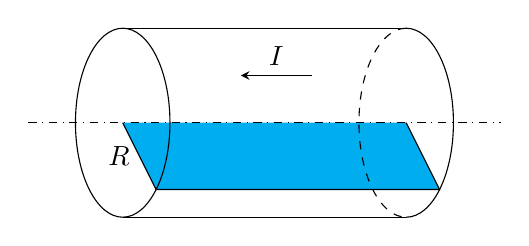
\begin{tikzpicture}[scale=0.6]
                [dashdotted/.style={dash pattern={on 15pt off 2pt on 2pt off 2pt}}]
                \draw[fill=cyan] (0,0) -- node[left]{\(R\)} ++(-45:1 and 2) -- ++(6,0) -- (6,0);
                \draw (0,0) ellipse (1 and 2);
                \draw[dashed] (6,0)++(90:1 and 2) arc (90:270:1 and 2);
                \draw (6,0)++(90:1 and 2) arc (90:-90:1 and 2);
                \draw (0,2) -- +(6,0);
                \draw (0,-2) -- +(6,0);
                \draw[dashdotted] (-2,0) --+(10,0);
                \draw[-stealth] (4,1) -- node[above]{\(I\)} (2.5,1);
            \end{tikzpicture}
            \caption{\ref{itm:20} 题图}
        \end{minipage}
    \end{figure}

    \item[7-22] 设有两无限大平行载流平面,它们的电流面密度均为\(j\),电流流向相反,求:(1)两载流平面之间的磁感强度;(2)两载流平面之外空间
        的磁感强度。
    
    \item[\mlabel{itm:26}{*7-26}] 如图所示,半径为\(R\)的圆片均匀带电,电荷面密度为\(\sigma\),令该圆片以角速度\(\omega\)绕通过其中心且垂直于圆片
        的轴旋转。求轴线上距圆片中心为\(x\)处的点P的磁感强度和旋转圆片的磁矩。
        \begin{figure}[htb]
            \centering
            \begin{minipage}[b]{0.4\textwidth}
                \centering
                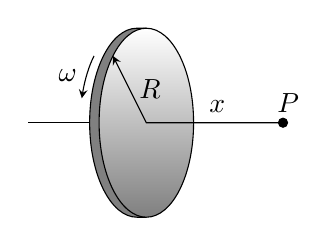
\begin{tikzpicture}[scale=0.6]
                    \draw (0,0) -- (-2.5,0);
                    \draw[fill=gray] (90:1 and 2) -- ++(-0.2,0) arc (90:270:1 and 2) -- ++(0.2,0);
                    \draw[top color= white,bottom color = gray] (0,0) ellipse (1 and 2);
                    \draw[Circle-stealth] (3,0) node[above]{\(P\)} -- node[above]{\(x\)} (0,0) -- node[right]{\(R\)} (135:1 and 2);
                    \draw[-stealth] (135:1 and 2)++(-0.4,0) arc (135:165:1 and 2) node[midway,left]{\(\omega\)};
                \end{tikzpicture}
                \caption{\ref{itm:26} 题图}
            \end{minipage}
            \begin{minipage}[b]{0.4\textwidth}
                \centering
                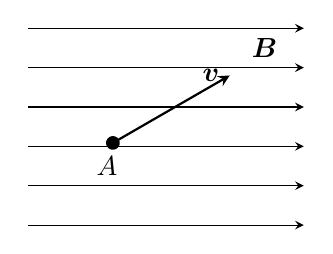
\begin{tikzpicture}
                    \foreach \x in {0,0.5,...,2.5}
                        \draw[-stealth] (0,\x) -- ++(3.5,0);
                    \draw[thick,Circle-stealth] (1,1) node[below]{\(A\)} -- ++(30:1.8) node[left]{\(\bm{v}\)};
                    \node[above] at (3,2) {\(\bm{B}\)};
                \end{tikzpicture}
                \caption{\ref{itm:29} 题图}
            \end{minipage}
        \end{figure}

    \item[\mlabel{itm:29}{7-29}] 如图所示,在\(B=\csi{0.01}{\tesla}\)的均匀磁场中,电子以\(v=\csi{e4}{\m\per\s}\)的速度在磁场中通过点\(A\)运动,
        电子运动速度和磁场\(\bm{B}\)的夹角为 \ang{30}。求电子的轨道半径和旋转频率。
        
    \item[\mlabel{itm:33}{7-33}] 霍耳效应可用来测量血流的速度,其原理如图所示。在动脉血管两侧分别安装电极并加以磁场。
        设血管直径为\csi{2.0}{\mm},磁感强度为\csi{0.080}{\tesla},毫伏表测出血管上下两端的电压为\csi{0.10}{\mV},
        则血流的速度为多大?
        \begin{figure}[htb]
            \centering
            \begin{minipage}[b]{0.4\textwidth}
                \centering
                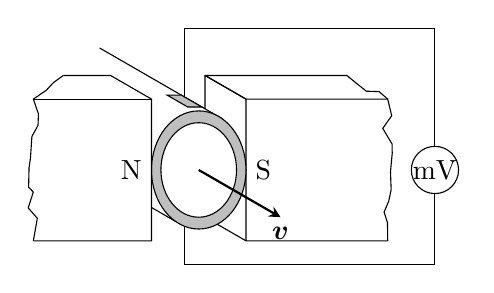
\begin{tikzpicture}[decoration={random steps,segment length=5pt,amplitude=2pt},scale=0.6]
                    \draw (-0.3,3) rectangle (5,-2);
                    \draw[fill=white] (5,0) circle (0.5) node{\(\mathrm{mV}\)};
                    \draw[join = round] (4,-1.5) coordinate (D) -- ++(-3,0) -- node[right]{S} ++(0,3) -- ++(150:1) -- ++(3,0) coordinate (E);
                    \draw[join = round] (1,-1.5) -- ++(150:1) -- ++(0,3) -- ++(-30:1) -- ++(3,0) coordinate (F);
                    \draw[decorate] (D) -- (F) -- (E);
                    \draw[fill=white] (60:1 and 1.25)++(150:3) -- ++(-30:3) -- ++(240:2 and 2.5) -- ++(150:3);
                    \draw[fill=lightgray] (0,0) ellipse (1 and 1.25);
                    \draw[fill=white] (0,0) ellipse (0.8 and 1);
                    \draw[fill=lightgray] (60:1 and 1.25)++(150:0.5) -- ++(-0.3,0) -- ++(150:0.5) -- ++(0.3,0) --cycle;
                    \draw[fill=white] (-3.5,-1.5) coordinate (C) -- ++(2.5,0) --node[left]{N} ++(0,3) -- ++(150:1) -- ++(-1,0) coordinate (A);
                    \draw (-1,1.5) -- ++(-2.5,0) coordinate (B);
                    \draw[decorate] (A) -- (B) -- (C);
                    \draw[thick,-stealth] (0,0) -- (-30:2) node[below]{\(\bm{v}\)};
                \end{tikzpicture}
                \caption{\ref{itm:33} 题图}
            \end{minipage}
        \end{figure}
    
    \item[7-35] 带电粒子在过饱和液体中运动会留下一串气泡,显示出粒子运动的径迹。设在气泡室中,有一个质子垂直于磁场飞过,
        留下一个半径为\csi{3.5}{\cm}的圆弧径迹,测得磁感强度为\csi{0.20}{\tesla},求此质子的动量和能量。
    
    \item[\mlabel{itm:37}{7-37}] 如图所示,一根长直导线载有电流\(I_1=\csi{30}{\A}\),矩形回路载有电流\(I_2=\csi{20}{\A}\)。
        试计算作用在回路上的合力。已知\(d=\csi{1.0}{\cm},b=\csi{8.0}{\cm},l=\csi{0.12}{\m}\)。
    
        \begin{figure}[htb]
            \centering
            \begin{minipage}[b]{0.4\textwidth}
                \centering
                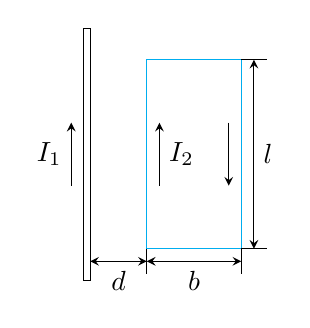
\begin{tikzpicture}[scale=0.8]
                    \draw (0,-2) rectangle (0.1,2);
                    \draw[cyan] (1,-1.5) rectangle (2.5,1.5);
                    \draw[-stealth] (-0.2,-0.5) -- node[left]{\(I_1\)} (-0.2,0.5);
                    \draw[-stealth] (1.2,-0.5) --node[right]{\(I_2\)} (1.2,0.5);
                    \draw[-stealth] (2.3,0.5) -- (2.3,-0.5);
                    \draw[thin] (2.5,1.5) -- ++(0.4,0);
                    \draw[thin] (2.5,-1.5) -- ++(0.4,0);
                    \draw[stealth-stealth] (2.7,-1.5) -- node[right]{\(l\)} (2.7,1.5);
                    \draw[thin] (1,-1.5) -- ++(0,-0.4);
                    \draw[thin] (2.5,-1.5) -- ++(0,-0.4);
                    \draw[stealth-stealth] (2.5,-1.7) -- node[below]{\(b\)} (1,-1.7);
                    \draw[stealth-stealth] (1,-1.7) -- node[below]{\(d\)} (0.1,-1.7);
                \end{tikzpicture}
                \caption{\ref{itm:37} 题图}
            \end{minipage}
            \begin{minipage}[b]{0.4\textwidth}
                \centering
                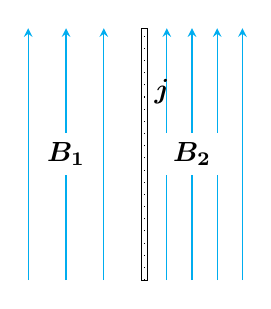
\begin{tikzpicture}[scale=0.8]
                    \foreach \x in {0,0.6,1.2}
                        \draw[-stealth,cyan] (\x,0) -- ++(0,4);
                    \foreach \x in {2.2,2.6,3.0,3.4}
                        \draw[-stealth,cyan] (\x,0) -- ++(0,4);
                    \draw (1.8,0) rectangle (1.9,4);
                    \draw[loosely dotted] (1.85,0) -- ++(0,4) node[near end,right]{\(\bm{j}\)};
                    \node[fill=white] at (0.6,2) {\(\bm{B_1}\)};
                    \node[fill=white] at (2.6,2) {\(\bm{B_2}\)};
                \end{tikzpicture}
                \caption{\ref{itm:39} 题图}
            \end{minipage}
        \end{figure}

    \item[\mlabel{itm:39}{7-39}] 将一电流均匀分布的无限大载流平面放入磁感强度为\(\bm{B}_0\)的均匀磁场中,电流方向与磁场垂直,放入后,
        平面两侧磁场的磁感强度分别为\(\bm{B}_1\)和\(\bm{B}_2\),如图所示。求该载流平面上单位面积所受的磁场力的大小和方向。
    
    \item[\mlabel{itm:41}{*7-41}] 如图所示,一根长直同轴电缆内、外导体之间充满磁介质,磁介质的相对磁导率为\(\mu_r\)(\(\mu_r>1\)),
        导体的磁化可以略去不计。电缆沿轴向有恒定电流I通过,内外导体上的电流的方向相反。求:(1)空间各区域内的磁感强度和磁化强度;
        *\negthickspace(2)磁介质表面的磁化电流。
        \begin{figure}[htb]
            \centering
            \begin{minipage}[b]{0.4\textwidth}
                \centering
                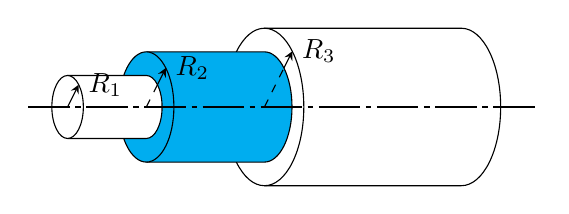
\begin{tikzpicture}
                    [dashdotted/.style={dash pattern={on 15pt off 2pt on 2pt off 2pt}}]
                    \draw (90:0.5 and 1) -- ++(2.5,0) arc (90:-90:0.5 and 1) -- ++(-2.5,0);
                    \draw (0,0) ellipse (0.5 and 1);
                    \draw[fill=cyan] (-1.5,0)++(90:0.35 and 0.7) -- ++(1.5,0) arc (90:-90:0.35 and 0.7) -- ++(-1.5,0);
                    \draw[fill=cyan] (-1.5,0) ellipse (0.35 and 0.7);
                    \draw[fill=white] (-2.5,0)++(90:0.2 and 0.4) -- ++(1,0) arc (90:-90:0.2 and 0.4) -- ++(-1,0);
                    \draw[fill=white] (-2.5,0) ellipse (0.2 and 0.4);
                    \draw[dashdotted] (-3,0) -- (3.5,0);
                    \draw[dashed] (0,0) -- (45:0.35 and 0.7);
                    \draw[-stealth] (45:0.35 and 0.7) -- (45:0.5 and 1) node[right]{\(R_3\)};
                    \draw[dashed] (-1.5,0) -- ++(45:0.2 and 0.4);
                    \draw[-stealth] (-1.5,0)++(45:0.2 and 0.4) -- ++(45:0.15 and 0.3) node[right]{\(R_2\)};
                    \draw[-stealth] (-2.5,0) -- ++(45:0.2 and 0.4) node[right]{\(R_1\)};
                \end{tikzpicture}
                \caption{\ref{itm:41} 题图}
            \end{minipage}
        \end{figure}
        
    \item[7-43] 在实验室中,为了测试某种磁性材料的相对磁导率\(\mu_r\),常将这种材料做成截面为矩形的圆环形样品,然后用漆包线绕成一螺线环。
        设圆环的平均周长为\csi{0.10}{\m},横截面积为\csi{0.5e-4}{\square\m},线圈共绕了\csi{200}{}匝。当线圈通过\csi{0.10}{\A}
        的电流时,测得穿过圆环横截面的磁通量为\csi{6.0e-8}{\weber},求此时该材料的相对磁导率\(\mu_r\)。
    
    \item 一边长为\(2a\)的载流正方形线圈,通有电流\(I\)。试求轴线上距正方形中心为\(r_0\)处的磁感强度,并证明当\(r_0\)远大于\(a\)时,
        磁感强度\(B=\frac{\mu_0m}{2\uppi r_0^3}\)。

    \item \label{itm:s2} 电流均匀流过宽为\(2a\)的无限长平面导体薄板,电流大小为\(I\),通过板的中线并与板面垂直的平面上有一点\(P\),\(P\)到板的垂直距离为\(x\)(如图),
        设板厚可略去不计,求\(P\)点的磁感强度。
        \begin{figure}[htb]
            \centering
            \begin{minipage}[b]{0.4\textwidth}
                \centering
                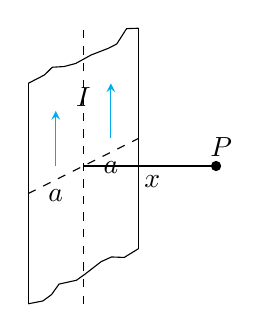
\begin{tikzpicture}[decoration={random steps,segment length=5pt,amplitude=2pt},scale=0.7]
                    \draw (0,0) -- (0,4);
                    \draw (2,1) -- (2,5);
                    \draw[decorate] (0,4) -- (2,5);
                    \draw[decorate] (0,0) -- (2,1);
                    \draw[thin,dashed] (0,2) -- node[below]{\(a\)} (1,2.5) --node[below]{\(a\)} (2,3);
                    \draw[dashed] (1,0) -- (1,5) node[near end]{\(I\)};
                    \draw[-Circle] (1,2.5) -- node[below]{\(x\)} (3.5,2.5) node[above]{\(P\)};
                    \draw[-stealth,thin,cyan] (0.5,2.5) -- (0.5,3.5);
                    \draw[-stealth,thin,cyan] (1.5,3) -- (1.5,4);
                \end{tikzpicture}
                \caption{\ref{itm:s2} 题图}
            \end{minipage}
            \begin{minipage}[b]{0.4\textwidth}
                \centering
                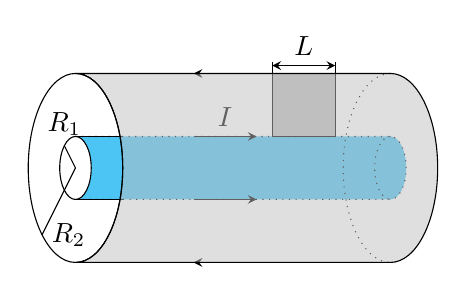
\begin{tikzpicture}
                    \draw[dotted, fill=cyan, fill opacity=0.7] (0,0.4) -- ++(4,0) arc (90:-90:0.2 and 0.4) -- ++(-4,0); 
                    \draw[fill=white] (0,0) ellipse (0.2 and 0.4);
                    \draw (0,0.4) -- (0.6,0.4);
                    \draw (0,-0.4) -- (0.6,-0.4);
                    \draw[fill=lightgray] (2.5,0.4) rectangle (3.3,1.2);
                    \draw (2.5,1.2) -- ++(0,0.15);
                    \draw (3.3,1.2) -- ++(0,0.15);
                    \draw[stealth-stealth] (2.5,1.3) -- node[above]{\(L\)} (3.3,1.3);
                    \draw[dotted] (4,0)++(90:0.2 and 0.4) arc (90:270:0.2 and 0.4);
                    \draw[dotted] (4,0)++(90:0.6 and 1.2) arc (90:270:0.6 and 1.2);
                    \draw[-stealth] (1.5,0.4) -- node[above]{\(I\)} (2.3,0.4);
                    \draw[-stealth] (1.5,-0.4) -- (2.3,-0.4);
                    \draw[stealth-] (1.5,1.2) -- (2.5,1.2);
                    \draw[stealth-] (1.5,-1.2) -- (2.5,-1.2);
                    \draw[fill=lightgray,fill opacity=0.5] (0,1.2) -- (4,1.2) arc (90:-90:0.6 and 1.2) -- (0,-1.2) arc (-90:90:0.6 and 1.2); 
                    \draw (0,0) ellipse (0.6 and 1.2);
                    \draw (0,0) -- (135:0.2 and 0.4) node[above]{\(R_1\)};
                    \draw (0,0) -- (225:0.6 and 1.2) node[right]{\(R_2\)};
                \end{tikzpicture}
                \caption{\ref{itm:s3} 题图}
            \end{minipage}
        \end{figure}

    \item \label{itm:s3} 一对无穷长直的空心导体圆筒内,内外筒半径分别为\(R_1\)和\(R_2\)(筒壁厚度可以忽略)。电流\(I\)沿内筒流去,沿外筒流回(见本题图),
        (1)计算两筒间的磁感强度\(B\);(2)通过长度为\(L\)的一段截面(图中阴影区)的磁通量\(\varPhi_B\)。
        
    \item \label{itm:s4} 矩形截面的螺线环,螺线环总匝数为\(N\),载流大小为\(I\),尺寸见本题图,(1)求环内磁感应强度的分布;(2)求通过螺线环截面(图中阴影区)的磁通量。 
        \begin{figure}[htb]
            \centering
            \begin{minipage}[b]{0.4\textwidth}
                \centering
                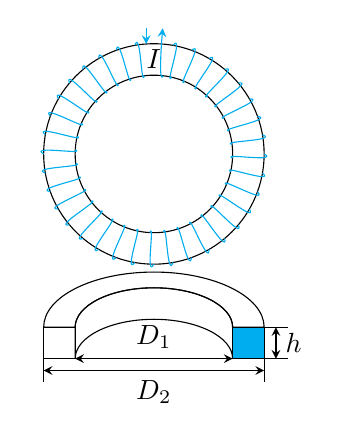
\begin{tikzpicture}
                    \draw (0,0) circle (1);
                    \draw (0,0) circle (1.4);
                    \foreach \x in {10,20,...,350}
                        \draw[rotate=\x,cyan] (90:1.4) .. controls (86:1.6) and (91:0.85) .. (87:1);
                    \draw[-stealth,cyan] (83:1) .. controls (87:0.85) and (86:1.6)  .. (86:1.6);
                    \node at (90:1.2) {\(I\)};
                    \draw[stealth-,cyan] (94:1.4) -- ++(0,0.2);
                    \draw (0,-2.2)++(0:1 and 0.5) arc (0:180:1 and 0.5) -- ++(0,-0.4) arc (180:0:1 and 0.5) --cycle;
                    \draw (0,-2.2)++(0:1.4 and 0.7) arc (0:180:1.4 and 0.7) --++(0.4,0) arc (180:0:1 and 0.5) --cycle;
                    \draw (0,-2.2)++(180:1.4 and 0.7) rectangle (-1,-2.6);
                    \draw[fill=cyan] (0,-2.2)++(1,0) rectangle (1.4,-2.6);
                    \draw[stealth-stealth] (-1,-2.6) -- node[above]{\(D_1\)} ++(2,0);
                    \draw[thin] (-1.4,-2.6) -- ++(0,-0.3);
                    \draw[thin] (1.4,-2.6) -- ++(0,-0.3);
                    \draw[thin] (1.4,-2.6) -- ++(0.3,0);
                    \draw[thin] (1.4,-2.2) -- ++(0.3,0);
                    \draw[stealth-stealth] (-1.4,-2.75) -- node[below]{\(D_2\)} ++(2.8,0);
                    \draw[stealth-stealth] (1.55,-2.2) -- node[right]{\(h\)} ++(0,-0.4);
                \end{tikzpicture}
                \caption{\ref{itm:s4} 题图}
            \end{minipage}
            \begin{minipage}[b]{0.4\textwidth}
                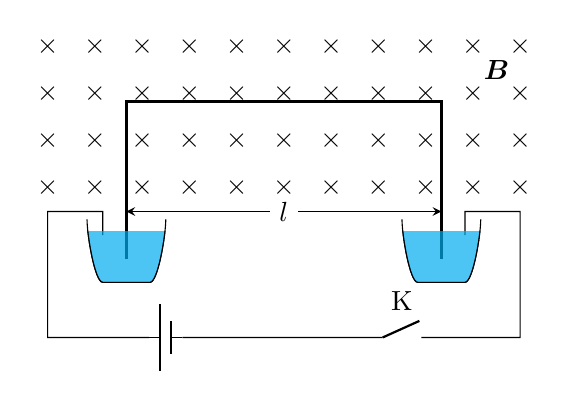
\begin{tikzpicture}
                    \draw[very thick] (-2,-2) -- (-2,0) -- (2,0) -- (2,-2);
                    \draw[stealth-stealth] (-2,-1.4) -- node[fill=white]{\(l\)} (2,-1.4);
                    \foreach \x in {-3,-2.4,...,3.6}
                        \foreach \y in {-1.1,-0.5,0.1,0.7}
                            \node at (\x,\y) {\(\times\)};
                    \node at (2.7,0.4) {\(\bm{B}\)};
                    \draw (-2.3,-1.7) -- (-2.3,-1.4) -- (-3,-1.4) -- (-3,-3) to[battery1] (0,-3) to[nos=K] (3,-3)
                        -- (3,-1.4) -- (2.3,-1.4) -- (2.3,-1.7);
                    \begin{scope}
                        \draw (-2.5,-1.5) .. controls (-2.5,-1.7) and (-2.4,-2.3) .. (-2.3,-2.3) -- 
                            (-1.7,-2.3) .. controls (-1.6,-2.3) and (-1.5,-1.7) .. (-1.5,-1.5);
                        \clip (-2.5,-1.65) rectangle (-1.5,-2.5);
                        \draw[fill=cyan,fill opacity=0.7] (-2.5,-1.5) .. controls (-2.5,-1.7) and (-2.4,-2.3) .. (-2.3,-2.3) -- 
                            (-1.7,-2.3) .. controls (-1.6,-2.3) and (-1.5,-1.7) .. (-1.5,-1.5);
                    \end{scope}
                    \begin{scope}[xshift=4 cm]
                        \draw (-2.5,-1.5) .. controls (-2.5,-1.7) and (-2.4,-2.3) .. (-2.3,-2.3) -- 
                            (-1.7,-2.3) .. controls (-1.6,-2.3) and (-1.5,-1.7) .. (-1.5,-1.5);
                        \clip (-2.5,-1.65) rectangle (-1.5,-2.5);
                        \draw[fill=cyan,fill opacity=0.7] (-2.5,-1.5) .. controls (-2.5,-1.7) and (-2.4,-2.3) .. (-2.3,-2.3) -- 
                            (-1.7,-2.3) .. controls (-1.6,-2.3) and (-1.5,-1.7) .. (-1.5,-1.5);
                    \end{scope}
                \end{tikzpicture}
                \caption{\ref{itm:s6} 题图}
            \end{minipage}
        \end{figure}

    \item 在一个显像管里,电子沿水平方向从南到北运动,动能是\csi{1.2e4}{\eV},该处地球磁场在竖直方向上的分量向下,\(\bm{B}\)的大小是\csi{5.5e-5}{\tesla},
        已知电子电荷\(-e=\csi{1.6e-19}{\coulomb}\),质量\(m=\csi{9.1e-31}{\kg}\)。(1)电子受地磁的影响往哪个方向偏转?(2)电子的加速度有多大?
        (3)电子在显像管内走\csi{20}{\cm}时,偏转有多大?(4)地磁对看电视有没有影响?

    \item \label{itm:s6} 一段导线弯成如图中所示的形状,它的质量是\(m\),上面水平一段的长度为\(l\),处在均匀磁场中,磁感强度为\(\bm{B}\),\(\bm{B}\)与导线垂直;
        导线下面两端分别插在两个浅水银槽里,两槽水银与一带开关K的外电源连接。当K一接通,导线便从水银槽里跳起来。
        (1)设跳起来的高度为\(h\),求通过导线的电量\(q\);(2)当\(m=\csi{10}{\g},l=\csi{20}{\cm},h=\csi{3.0}{\m},B=\csi{0.10}{\tesla}\)时,求\(q\)的量值。
        \begin{figure}[htb]
            \centering
            \begin{minipage}[b]{0.4\textwidth}
                \centering
                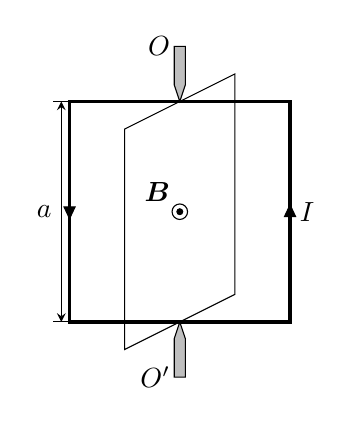
\begin{tikzpicture}[scale=0.7]
                    \draw[very thick] (-2,2) rectangle (2,-2);
                    \node[currarrow,rotate=-90] at (-2,0){};
                    \node[currarrow,rotate=90] at (2,0){};
                    \draw[fill] (0,0) circle (1.5pt);
                    \draw (0,0) circle (4pt);
                    \node[above left] at (0,0) {\(\bm{B}\)};
                    \draw (-1,1.5) -- (1,2.5) -- (1,-1.5) -- (-1,-2.5) --cycle;
                    \draw (-2,2) -- ++(-0.3,0) (-2,-2) -- ++(-0.3,0);
                    \draw[stealth-stealth] (-2.15,2) -- node[left]{\(a\)} ++(0,-4);
                    \node[right] at (2,0) {\(I\)};
                    \draw[fill=lightgray] (0,2) -- (0.1,2.3) -- (0.1,3) -- node[left]{\(O\)} (-0.1,3) -- (-0.1,2.3) -- cycle;
                    \draw[fill=lightgray] (0,-2) -- (0.1,-2.3) -- (0.1,-3) -- node[left]{\(O^\prime\)} (-0.1,-3) -- (-0.1,-2.3) -- cycle;
                \end{tikzpicture}
                \caption{\ref{itm:s7} 题图}
            \end{minipage}
            \begin{minipage}[b]{0.4\textwidth}
                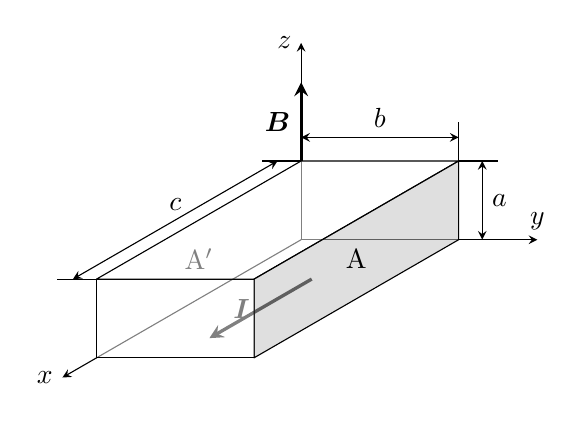
\begin{tikzpicture}[join = round]
                    \draw[-stealth] (0,0) -- (210:3.5) node[left]{\(x\)};
                    \draw[-stealth] (0,0) -- (3,0) node[above]{\(y\)};
                    \draw[-stealth] (0,0) -- (0,2.5) node[left]{\(z\)};
                    \draw[very thick,-stealth] (210:1)++(1,0) --node[left]{\(\bm{I}\)} ++(210:1.5);
                    \node[yshift=0.5cm] at (210:1.5) {\(\mathrm{A^\prime}\)};
                    \draw[fill=white,fill opacity=0.5] (210:3) rectangle ++(2,1);
                    \draw[fill=white,fill opacity=0.5] (210:3)++(0,1) -- ++(30:3) -- ++(2,0) -- ++(210:3) -- cycle;
                    \draw[fill=lightgray,fill opacity=0.5] (210:3) ++(2,0) -- ++(0,1) -- ++(30:3) -- ++(0,-1) -- ++(210:3) -- cycle;
                    \node[xshift=2cm,yshift=0.5cm] at (210:1.5) {\(\mathrm{A}\)};
                    \draw[very thick,-stealth] (0,1) -- node[left]{\(\bm{B}\)} (0,2);
                    \draw[thin] (2,1) -- ++(0,0.5) (2,1) -- ++(0.5,0) (0,1) -- ++(-0.5,0) (210:3)++(0,1) -- ++(-0.5,0);
                    \draw[thin,stealth-stealth] (0,1.3) --node[above]{\(b\)} (2,1.3) ;
                    \draw[thin,stealth-stealth] (2.3,1) --node[right]{\(a\)} (2.3,0) ;
                    \draw[thin,stealth-stealth] (-0.3,1) --node[above]{\(c\)} ++(210:3);
                \end{tikzpicture}
                \caption{\ref{itm:s8} 题图}
            \end{minipage}
        \end{figure}

    \item \label{itm:s7} 一边长为\(a\)的正方形线圈载有电流\(I\),处在均匀外磁场\(\bm{B}\)中,\(\bm{B}\)垂直于纸面向外,线圈可以绕通过中心的竖直轴\(OO^\prime\)转动(见本题图),
        转动惯量为\(J\),求线圈在平衡位置附近作微小摆动(\(\sin\theta\approx\theta\),简谐振动)的周期\(T\)。

    \item \label{itm:s8} 一块半导体样品的体积为\(a\times b\times c\),如图所示,沿\(x\)方向有电流\(I\),在\(z\)轴方向加有均匀磁场\(\bm{B}\),实验数据为
        \(a=\csi{0.10}{\cm}, b=\csi{0.35}{\cm},c=\csi{1.0}{\cm}, I=\csi{1.0}{\mA}, B=\csi{0.3}{\tesla}\),片两侧的电势差为\(U_{AA^\prime}=\csi{6.55}{\mV}\),
        (1)问这半导体是正电荷导电(P型)还是负电荷导电(N型)?(2)求载流子浓度(即单位体积内参加导电的带电粒子数)。
        

    \item \label{itm:s9} 一磁导率为\(\mu_1\)的无限长圆柱形直导线,半径为\(R_1\),其中均匀地通有电流\(I\)。 在导线外包一层磁导率为\(\mu_2\)的圆柱形不导电的磁介质,
        其外半径为\(R_2\),如图所示。试求:(1) 磁场强度和磁感强度的分布;(2) 半径为\(R_1\)和\(R_2\)处表面上磁化电流面密度。
        \begin{figure}[htb]
            \centering
            \begin{minipage}[b]{0.5\textwidth}
                \centering
                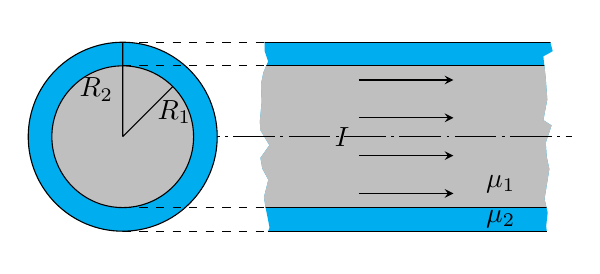
\begin{tikzpicture}[decoration={random steps,segment length=5pt,amplitude=2pt},scale=0.6]
                    \begin{scope}
                        \clip[decorate] (3,2.2) rectangle (9,-2.2);
                        \draw[fill=cyan] (2.5,2) rectangle (10,-2);
                        \draw[fill=lightgray] (2.5,1.5) rectangle (10,-1.5);
                    \end{scope}
                    \draw[dash pattern={on 15pt off 2pt on 1pt off 2pt}] (0,0) -- (9.5,0);
                    \draw[fill=cyan] (0,0) circle (2);
                    \draw[fill=lightgray] (0,0) circle (1.5);
                    \draw[dashed] (0,1.5) -- (3,1.5) (0,2) -- (3,2) (0,-1.5) -- (3,-1.5) (0,-2) -- (3,-2);
                    \draw (0,0) -- node[right]{\(R_1\)} (45:1.5) (0,0) --node[left]{\(R_2\)} (90:2);
                    \node at (8,-1) {\(\mu_1\)};
                    \node at (8,-1.75) {\(\mu_2\)};
                    \foreach \x in {1.2,0.4,-0.4,-1.2}
                        \draw[-stealth] (5,\x) -- ++(2,0);
                    \node[left] at (5,0) {\(I\)};
                \end{tikzpicture}
                \caption{\ref{itm:s9} 题图}
            \end{minipage}
        \end{figure}
\end{enumerate}
\end{document} 